%%%%%%%%%%%%%%%%%%%%%%%%%%%%%%%%%
\newpage
%%%%%%%%%%%%%%%%%%%%%%%%%%%%%%%%%
\section{Convolution introduction}

\subsection*{Resources}
\begin{itemize}
    \item Video lecture 8 starting at 32:15: \url{https://youtu.be/wUT1huREHJM?t=32m15s}
    \item Book: Chapter 3.1 (\url{https://see.stanford.edu/materials/lsoftaee261/book-fall-07.pdf})
\end{itemize}

\subsection*{Comment}
Here we expand our study to convolution; a powerful function for processing signals.
This introduction by Prof. Osgood provides an excellent introduction.
What you will learn here is that convolution in real space is related to multiplication in frequency space.
Visualisation of what convolution in real-space means however, is rather difficult, and I would recommend to focus purely on the mathematical meaning here of how it relates functions in real space and frequency space.

\subsection*{Challenge}
Briefly describe what convolution of two functions means, and how it can relate two functions of time in real space to their equivalent functions in frequency space.

Show that convolution in real-space ($\ff(g*f)(s)$) corresponds to multiplication in frequency space ($\ff g(s) \ff f(s)$).

\subsection*{Solution}
Please compare your answer with your partner or discuss with the teacher in class.




%%%%%%%%%%%%%%%%%%%%%%%%%%%%%%%%%
\newpage
%%%%%%%%%%%%%%%%%%%%%%%%%%%%%%%%%
\section{Filtering}

\subsection*{Resources}
\begin{itemize}
    \item Video lecture 9 until 24:15: \url{https://www.youtube.com/watch?v=NrOR2qMVWOs}
\end{itemize}

\subsection*{Comment}
The above video includes an excellent example of using fourier analysis in a scientific context, including its application in filters. I encorage you to watch until 24:15. After this point Prof. Osgood goes on to describe the futility of trying to visualise convolution in the time-domain, however the graphics on convolution on Wikipedia [1] (especially these: [2a,b]) I think go a little way to visualising what's happening in the time-domain.

1: \url{https://en.wikipedia.org/wiki/Convolution}\\
2a: \url{https://en.wikipedia.org/wiki/Convolution\#/media/File:Convolution_of_box_signal_with_itself2.gif}\\
2b: \url{https://en.wikipedia.org/wiki/Convolution\#/media/File:Convolution_of_spiky_function_with_box2.gif}

For your reference, turbidity standards of 5, 50, and 500 Nephelometric Turbidity Units (left to right respectively) are shown here:\\
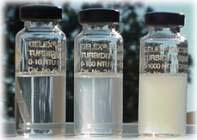
\includegraphics{turbidity.png}\\
\emph{Source: \url{https://en.wikipedia.org/wiki/Turbidity}}

\subsection*{Challenge}
%1. Take notes following the above video until 24:15. There is a lot of useful information here. The questions below highlight the key points that I want you to understand, however they do not cover everything, so please be sure to follow the video.

Using a few sentences and diagrams, describe an ideal low-pass, high-pass and band-pass filter. How can they be applied in the frequency domain to influence the signal in the time-domain?

\subsection*{Solution}
Please compare your answer with your partner or discuss with the teacher in class.




%%%%%%%%%%%%%%%%%%%%%%%%%%%%%%%%%
\newpage
%%%%%%%%%%%%%%%%%%%%%%%%%%%%%%%%%
\section{Convolution with a window function}

\subsection*{Comment}
The ``signal'' here is $g(t-\tau)$ and the ``window function'' is $f(\tau)$.

\subsection*{Challenge}
%1. Consider that you have a (somewhat unrealistic but mathematically manageable) input signal that varies as $g(t-\tau)=(t-\tau)^2$ with time. 
Consider that you have a (somewhat unrealistic but mathematically manageable) input signal that varies as $g(t)=t^2$ with time. 

Obtain the convolution of the signal $(f \star g)(t)$ with a window function:
\begin{equation}
    f(t)=
    \begin{cases}
        1 & \text{for } -1/2 < t < 1/2\\
        0 & \text{otherwise}
    \end{cases}
\end{equation}

%2. If this window-function were a filter, what sort of band-pass filter could you consider this to be?

\subsection*{Solution}
Your answer should be consistent with $(f \star g)(2) = 49/12$




%%%%%%%%%%%%%%%%%%%%%%%%%%%%%%%%%
\newpage
%%%%%%%%%%%%%%%%%%%%%%%%%%%%%%%%%
\section{Convolution with a continuous function}

\subsection*{Challenge}
Calculate the convolution of $f(t)=t$ with $g(t)=e^{-|t|}$.

\emph{Hint 1: $\int_{-\infty}^{\infty} \text{(even function)} = 2 \int_{0}^{\infty} \text{(even function)}$.}

\emph{Hint 2: It does not matter which function you make ``f'' or ``g'', but one way is easier than the other to compute.}

\subsection*{Solution}
To check your answer, substitute $t=1$ into your final answer and you should obtain $(f \star g)(1) = 2$.




%%%%%%%%%%%%%%%%%%%%%%%%%%%%%%%%%%
%\newpage
%%%%%%%%%%%%%%%%%%%%%%%%%%%%%%%%%%
%\section{Inequalities}
%
%\subsection*{Challenge}
%1. Re-write $-1/2 < t - \tau$ in the form $f(\tau) < t$ replacing $f(\tau)$ with appropriate expressions.
%
%2. Re-write $t - \tau < 1/2$ in the form $t < f(\tau)$ replacing $f(\tau)$ with appropriate expressions.
%
%3. Re-write $-1/2 < t - \tau < 1/2$ in the form $f(\tau) < t < g(\tau)$ replacing $f(\tau)$ and $g(\tau)$ with appropriate expressions.
%
%\subsection*{Solution}
%To check your solutions, substitute $\tau=1/2$ into the final expressions:
%
%1. $f(1/2)$: \hash{kkk}{115edb}\\
%2. $f(1/2)$: \hash{mmm}{6d64cd}\\
%3. $f(1/2)$: \hash{nnn}{414d80} and $g(1/2)$: \hash{ooo}{3ec4d7}




%%%%%%%%%%%%%%%%%%%%%%%%%%%%%%%%%%
%\newpage
%%%%%%%%%%%%%%%%%%%%%%%%%%%%%%%%%%
%\section{Touching window functions}
%\label{sec:touchingwindows}
%
%\subsection*{Challenge}
%1. Consider two window functions $f$ and $g$.
%\begin{equation}
%    f(\tau)=
%    \begin{cases}
%        1 & \text{for } -1/2 < \tau < 1/2\\
%        0 & \text{otherwise}
%    \end{cases}
%\end{equation}
%\begin{equation}
%    g(t-\tau)=
%    \begin{cases}
%        1 & \text{for } -1/2 < t-\tau < 1/2\\
%        0 & \text{otherwise}
%    \end{cases}
%\end{equation}
%You can imagine a fixed window function $f$ and a shiftable window-function $g$ (depending on the value of $t$). What is the value of $t$ in the following situations?
%
%a) The left side of window $f$ and the right side of window $g$ are touching.\\
%b) Complete overlap of windows $f$ and $g$.\\
%c) The right side of window $f$ and the left side of window $g$ are touching.
%
%2.\\
%a) Write a function that describes the position of the left-hand-side of window function $g$ at time $t$.\\
%b) Write a function that describes the position of the right-hand-side of window function $g$ at time $t$.\\
%To check your answers, substitute $t=1$ into your expressions.
%
%\subsection*{Solution}
%1.a) \hash{rrr}{1e3803}\\
%1.b) \hash{sss}{171271}\\
%1.c) \hash{ttt}{95acc3}\\
%
%2.a) \hash{uuu}{e27eca}\\
%2.b) \hash{vvv}{23da5b}




%%%%%%%%%%%%%%%%%%%%%%%%%%%%%%%%%
\newpage
%%%%%%%%%%%%%%%%%%%%%%%%%%%%%%%%%
\section{Convolution of two window functions}

\subsection*{Challenge}
%1. Show that the convolution of the two window functions in challenge \ref{sec:touchingwindows} in the time-domain results in the triangle function
%\begin{equation}
%    h(t)=
%    \begin{cases}
%        1+t & \text{for } 1 < t < 0\\
%        1-t & \text{for } 0 < t < 1\\
%        0 & \text{otherwise}
%    \end{cases}
%\end{equation}

In challenge \ref{sec:tophat} you calculated the spectrum of a window function. Imagine here you have two window functions $f(t)$ and $g(t)$.

\begin{equation}
    f(t)=
    \begin{cases}
        1 & \text{for } |t| < 1/2 \\
        0 & \text{for } |t| > 1/2
    \end{cases}
\end{equation}

\begin{equation}
    g(t)=
    \begin{cases}
        1 & \text{for } |t| < 1/2 \\
        0 & \text{for } |t| > 1/2
    \end{cases}
\end{equation}

1. Use your knowledge of the window-function in the frequency domain from challenge \ref{sec:tophat} to calculate the frequency-domain spectrum of the convolution of the two window functions.

2. What is the resulting function in the time-domain? \emph{This should be possible by deduction based on previous challenges, without calculation.}

\subsection*{Solution}
1. Substitute $s=1/2$ into your final answer and you should obtain 0.405.

2. Substitute $t=1/2$ into your final answer and you should obtain 0.50.

